\newpage

\section{Porównanie algorytmów detekcji twarzy}

W rozdziale \hyperref[{section:face_detection}]{\ref{section:face_detection}} przedstawiono kilka metod, które zostały zaimplementowane w~projekcie. Ze~względu, że~dla prawidłowego i~akceptowalnego działania aplikacji potrzebna jest odpowiednia skuteczność oraz szybkość detekcji twarzy wszystkie metody zostały przetestowane i~porównane (z wyłączeniem CNN MMOD - patrz rozdz. \hyperref[{section:no_cnn}]{\ref{section:no_cnn}}). Na podstawie wyników została wybrana jedna, która używana jest w~finalnej części projektu.


\subsection{Odrzucenie algorytmu CNN} \label{section:no_cnn}

Ze względu na bardzo wolne działanie algorytmu opartego na konwolucyjnych sieciach neuronowych został on wykluczony z~testów. Czas przetwarzania jednego zdjęcia 500x500 wynosił kilka sekund, co całkowicie uniemożliwia działanie aplikacji w~czasie rzeczywistym. Bardzo niska prędkość detekcji prawdopodobnie wynika z~niemożności skorzystania z~obliczeń na karcie graficznej na urządzeniach mobilnych. Metoda ta jest bardzo szybka gdy wykorzystuje do działania takie architektury jak CUDA \cite{nvidia_cuda}, natomiast dużo gorzej radzi sobie z~obliczeniami wykonywanymi na procesorach CPU.

\subsection{Testowanie na statycznych zdjęciach}

Pierwszy etap testowania algorytmów detekcji twarzy bazował na statycznych zdjęciach z~głównego zbioru danych (rozdz. \hyperref[section:dataset]{\ref{section:dataset}}). Pozwoliło to przetestować na jednakowych danych wszystkie metody pod względem ich skuteczności wykrywania docelowych obszarów w różnych warunkach oraz uzyskać miarodajne wyniki.

\subsubsection{Oczekiwany wynik}

Każde zdjęcie z~przygotowanego zbioru zostało opisane przez dwa prostokąty między którymi powinna się znaleźć wykryta przez algorytm twarz. Obszar ten został dobrany w~następujący sposób:

\begin{itemize}
    \item Wewnętrzna część obejmuje minimalny obszar, na którym znajdują się brwi, oczy, nos i~usta.
    \item W zewnętrznym prostokącie powinna znaleźć się cała twarz. Powiększony jest on o~pewną tolerancję. 
\end{itemize}

\begin{figure}[!h]
    \begin{center}
        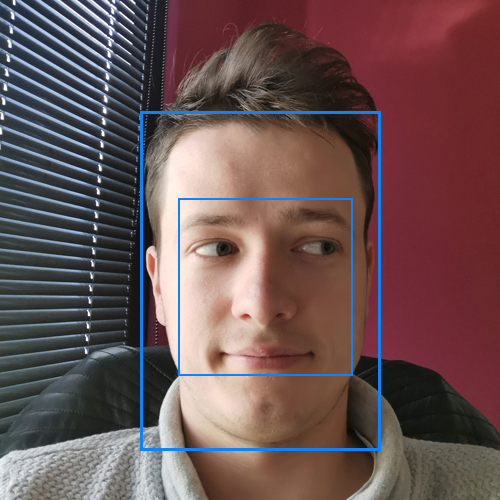
\includegraphics[scale=0.3]{img/face_section/face_test_expected.jpg}
        \caption{Oczekiwany obszar detekcji twarzy. }
        \label{fig:face_test_expected}
    \end{center}
\end{figure}

\subsubsection{Warunki testowania}

Dla każdego algorytmu zostały przeprowadzone testy na zestawach obrazów o~następujących rozdzielczościach i~przestrzeniach barw:

\begin{itemize}
    \item 300x300 RGB
    \item 500x500 RGB
    \item 300x300 skala szarości
    \item 500x500 skala szarości
\end{itemize}

W przypadku DNN Caffe nie było możliwe przeprowadzenie badań dla zdjęć w~skali szarości, ponieważ wymaga on obrazu w~trójkanałowej przestrzeni barw.

\par

Testy wykonywane były w~trybie \textit{wydaniowym (ang. release)}, ponieważ w~trybie \textit{debuggowania} algorytm Dlib HOG działał nawet $180$ razy wolniej. W przypadku pozostałych algorytmów tryb budowania nie miał większego wpływu na prędkość obliczeń, ale żeby wyniki były jak najbardziej miarodajne to każdy test musiał być przeprowadzony w~tych samych warunkach.







\subsubsection{Badanie skuteczności detekcji} \label{section:skutecznosc_detekcji_twarzy}

W~tym teście zostały zebrane i~porównane następujące dane:
\begin{itemize}
    \item \textbf{Prawidłowe detekcje} - suma perfekcyjnych i~częściowo dobrych detekcji
    \item \textbf{Perfekcyjne detekcje} - jeśli wykryty obszar w~pełni znajduje się pomiędzy oczekiwanym prostokątami
    \item \textbf{Częściowo dobre detekcje} - jeśli są krawędzie, które znajdują się poza oczekiwanym obszarem, ale w~zadowalającej odległości (patrz niżej - \hyperref[{uwaga:czesciowo_dobry}]{\textit{Uwaga 1.}})
    \item \textbf{W 3 na 4 krawędziach perfekcyjne detekcje} - jeśli tylko jedna krawędź znajduje się poza oczekiwanym obszarem w~zadowalającej odległości (patrz niżej - \hyperref[{uwaga:3_4_perfekcyjny}]{\textit{Uwaga 2.}})
    \item \textbf{Złe detekcje} - jeśli twarz nie została wykryta lub wskazany obszar jest niezadowalający
    \item \textbf{Twarze niewykryte} - jeśli całkowicie nie udało się wykryć twarzy (patrz niżej - \hyperref[{uwaga:dodatkowy_zle}]{\textit{Uwaga 3.}})
\end{itemize}

\textit{Uwaga 1.}\label{uwaga:czesciowo_dobry} Obszar uznawany jest za częściowo dobry jeśli żadna krawędź nie jest oddalona o~więcej niż $1.2x$ i maksymalnie jedna oddalona jest o~długość z przedziału $[1.1x, 1.2x]$. Odległość $x$ to szerokość lub wysokość (zależnie od krawędzi) maksymalnego oczekiwanego obszaru twarzy.

\par

\textit{Uwaga 2.}\label{uwaga:3_4_perfekcyjny} Obszar zaliczany jest do grupy 3/4 perfekcyjnych detekcji, jeśli 3 krawędzie znajdują się w~oczekiwanym obszarze, a czwarta odchylona jest od normy w przedziale $[1.0x, 1.2x]$.

\par 

\textit{Uwaga 3.}\label{uwaga:dodatkowy_zle} Dodatkowy podział złej detekcji na niewykryte twarze wynikał z~faktu, że~metody oparte o~Cascasding Classifier na wyjściu podają obszar kwadratowy i~przy rozciągniętej lub pochylonej twarzy boczne obszary mogą być bardzo oddalone od oczekiwanej wartości, ale dalej skutecznie wykrywać twarz. 

\vspace{10mm}

\begin{table}[!h]
\label{tab:face_detect_accuracy_RGB}
\centering
\caption{Skuteczność algorytmów detekcji twarzy dla obrazów RGB}
\resizebox{\textwidth}{!}{%
\begin{tabular}{|c|c|c|c|c|c|c|c|}
\hline
 &
  \textbf{\begin{tabular}[c]{@{}c@{}}Prawidłowe\\ detekcje\end{tabular}} &
  \textbf{\begin{tabular}[c]{@{}c@{}}Perfekcyjne\\ detekcje\end{tabular}} &
  \textbf{\begin{tabular}[c]{@{}c@{}}Częściowo\\ dobre\\ detekcje\end{tabular}} &
  \textbf{\begin{tabular}[c]{@{}c@{}}3/4\\ krawędzie\\ perfekcyjne\end{tabular}} &
  \textbf{\begin{tabular}[c]{@{}c@{}}Złe\\ detekcje\end{tabular}} &
  \textbf{\begin{tabular}[c]{@{}c@{}}Niewykryte\\ twarze\end{tabular}}  \\ \hline\hline
\textbf{Haar Cascade 500x500} &
  69 &
  4 &
  65 &
  32 &
  11 &
  9 \\ \hline
  
\textbf{Haar Cascade 300x300} &
 68 &
  5 &
  63 &
  33 &
  12 &
   9  \\ \hline
  
  \textbf{LBP Cascade 500x500} &
  58 &
  4 &
  54 &
  29 &
  22 &
  22 \\ \hline
  
  \textbf{LBP Cascade 300x300} &
  61 &
  4 &
  57 &
  34 &
  19 &
  17  \\ \hline
  
\textbf{DNN Caffe 500x500} &
  80 &
  68 &
  12 &
  11 &
  0 &
  0  \\ \hline
  
\textbf{DNN Caffe 300x300} &
  80 &
  62 &
  18 &
  18 &
  0 &
  0  \\  \hline
  
\textbf{Dlib HOG 500x500} &
  78 &
  31 &
  47 &
  36 &
  2 &
  2  \\  \hline
  
\textbf{Dlib HOG 300x300} &
  76 &
  24 &
  52 &
  33 &
  4 &
  4  \\  \hline
  
  \hline
\end{tabular}%
}
\end{table}
\begin{table}[!h]
\label{tab:face_detect_accuracy_GRAY}
\centering
\caption{Skuteczność algorytmów detekcji twarzy dla obrazów w skali szarości ze zbioru danych}
\resizebox{\textwidth}{!}{%
\begin{tabular}{|c|c|c|c|c|c|c|}
\hline
 &
  \textbf{\begin{tabular}[c]{@{}c@{}}Prawidłowe\\ detekcje\end{tabular}} &
  \textbf{\begin{tabular}[c]{@{}c@{}}Perfekcyjne\\ detekcje\end{tabular}} &
  \textbf{\begin{tabular}[c]{@{}c@{}}Częściowo\\ dobre\\ detekcje\end{tabular}} &
  \textbf{\begin{tabular}[c]{@{}c@{}}3/4\\ krawędzie\\ perfekcyjne\end{tabular}} &
  \textbf{\begin{tabular}[c]{@{}c@{}}Złe\\ detekcje\end{tabular}} &
  \textbf{\begin{tabular}[c]{@{}c@{}}Niewykryte\\ twarze\end{tabular}}   \\ \hline \hline
\textbf{Haar Cascade 500x500} &
  69 &
  4 &
  65 &
  31 &
  11 &
  9  \\ \hline

\textbf{Haar Cascade 300x300} &
  67 &
  4 &
  63 &
  34 &
  13 &
  9  \\ \hline
  
\textbf{LBP Cascade 500x500} &
  60 &
  5 &
  55 &
  30 &
  20 &
  17  \\ \hline
  
\textbf{LBP Cascade 300x300} &
  60 &
  4 &
  56 &
  31 &
  20 &
  17  \\ \hline
  
\textbf{DNN Caffe 500x500} &
  nd. &
  nd. &
  nd. &
  nd. &
  nd. &
  nd. \\ \hline
  
\textbf{DNN Caffe 300x300} &
  nd. &
  nd. &
  nd. &
  nd. &
  nd. &
  nd.  \\ \hline
  
  \textbf{Dlib HOG 500x500} &
  75 &
  27 &
  48 &
  35 &
  5 &
  5  \\ \hline
  
\textbf{Dlib HOG 300x300} &
  72 &
  23 &
  49 &
  31 &
  7 &
  7  \\ \hline
  
  \hline
\end{tabular}%
}
\end{table}

Metoda Haar Cascade pozwoliła uzyskać średnio $\sim69/80$ $(86\%)$ dobrych detekcji. Jest to relatywnie przeciętny wynik. Na taki rezultat składa się kilka problemów tej metody. Nie radzi sobie ona dobrze z~częściowo zakrytymi twarzami lub gdy głowa jest pochylona w bok. Kolejnymi czynnikiem wpływającym negatywnie na detekcje jest światło - problem z~wykrywaniem występuje gdy zdjęcie jest zbyt jasne, twarz oświetlona lub źródło światła świeci prosto w obiektyw. Zaletą tej metody jest mała ilość zwróconych przez nią dodatkowych, błędnych obszarów, które musiały zostać odfiltrowane.

\par

\textit{Klasyfikator kaskadowy} bazując na modelu LBP miał najgorsze wyniki detekcji twarzy, na poziomie $\sim60/80$ $(75 \%)$. Jednak co zwraca uwagę to fakt, że~bardzo duży odsetek twarzy nie został w~ogóle wykryty. Występują tu te same problemy co~w~Haar Cascade, ale~dodatkowo algorytm nie radzi sobie gdy twarz zajmuje dużą część zdjęcia.

\par

Najlepszy wynik detekcji uzyskał bezdyskusyjnie DNN Caffe. Fakt, że~w~każdym z~dwóch testów wykrył on $100 \%$ twarzy jest warty odnotowania. Co więcej, perfekcyjne detekcje były na poziomie $\sim65/80$ $(81,25 \%)$. Nie występują tu problemy takie jak w~poprzednich algorytmach. Radzi sobie on dobrze nawet w~złych warunkach oświetleniowych. Częściowe zakrycie twarzy nie wpływa w~znacznym stopniu na detekcję. Wykrywa on dobrze zarówno pochylone jak i~odwrócone twarze. Jedynym negatywnym zjawiskiem, które udało się zaobserwować w~tej metodzie to zwracanie wielu dodatkowych obszarów, które są błędne. Zastosowanie filtrowania pozwoliło jednak odrzucić wszystkie błędne wskazania.

\par

Bardzo dobre wyniki detekcji uzyskał również algorytm Dlib HOG, w~szczególności w~przypadku zdjęć RGB 500x500 - jego skuteczność była na poziomie $78/80$ $(97,5 \%$). Zaletą tej metody jest zwracanie tylko jednego wykrytego obszaru - na żadnym z~80 zdjęć nie zwrócił ani jednego dodatkowego miejsca, które uznał za twarz. Nie wykrył on twarzy gdy była w~połowie zasłonięta. Zakładając jednak, że~aplikacja będzie analizować twarz użytkownika korzystającego z~telefonu można przyjąć, że będzie ona w~wystarczającym stopniu widoczna. W~przeciwieństwie do pozostałych metod, które zwracają obszar całej twarzy, ta wykrywa częściowo obcięty rejon - np. pomijając czoło. Nie jest to w~ogólności wadą, ponieważ te elementy nie są wykorzystywane w~projekcie pracy dyplomowej.

\vspace{5mm}

Różnica w~procencie perfekcyjnych detekcji pomiędzy DNN Caffe, a~pozostałymi metodami wynika z rodzaju zwracanych przez nie obszarów. Metoda oparta na głębokich sieciach neuronowych zwraca prostokąt o~dowolnym stosunku boków, natomiast reszta zwraca kwadrat. Dzięki temu DNN lepiej dopasowuję się do kształtu twarzy niż Cascading Classifier i~HOG.

\vspace{5mm}

Zmiana przestrzeni barw nie wpłynęła istotnie na rezultaty poszczególnych algorytmów. Jedynie zauważalne było obniżenie skuteczności detekcji w~skali szarości w~porównaniu do RGB dla metody opartej na histogramie gradientów zorientowanych.







\subsubsection{Badanie szybkości detekcji}

W~tym teście zostały zebrane i~porównane następujące dane:

\begin{itemize}
    \item \textbf{Całkowity czas przetwarzania} - suma czasów wszystkich 20 iteracji, całkowity czas testu.
    \item \textbf{Średni czas przetwarzania pojedynczej iteracji} - uśredniony czas pojedynczej iteracji
    \item \textbf{Średni czas przetwarzania jednego zdjęcia} - uśredniony czas przetwarzania pojedynczego zdjęcia
\end{itemize}

\par
\textit{Uwaga 1.}\label{uwaga:ilosc_powtorzen} Celem miarodajnego wyniku czasu przetwarzania każdy test został przeprowadzony 20 razy.

\vspace{10mm}

\begin{table}[!h]
\label{tab:face_detect_speed_RGB}
\centering
\caption{Czas przetwarzania algorytmów detekcji twarzy dla obrazów RGB}

\begin{tabular}{|c|c|c|c|}
\hline
 & 
  \textbf{\begin{tabular}[c]{@{}c@{}}Całkowity czas \\ przetwarzania \end{tabular}} &
  \textbf{\begin{tabular}[c]{@{}c@{}}Średni czas\\ przetwarzania \\ pojedynczej iteracji\end{tabular}} &
  \textbf{\begin{tabular}[c]{@{}c@{}}Średni czas\\przetwarzania \\ pojedynczego\\zdjęcia\end{tabular}} \\ \hline\hline
\textbf{Haar Cascade 500x500} & 
  116,72 s &
  5,836 s &
  0,072 s    \\ \hline
  
\textbf{Haar Cascade 300x300} & 
  46,24 s &
  2,312 s &
  0,028 s     \\ \hline
  
  \textbf{LBP Cascade 500x500} & 
  63,27 s &
  3,163 s&
  0,039 s  \\ \hline
  
  \textbf{LBP Cascade 300x300} & 
  21,25 s &
  1,062 s &
  0,013 s    \\ \hline
  
\textbf{DNN Caffe 500x500} &
  106,17 &
  5,308 &
  0,066 s  \\ \hline
  
\textbf{DNN Caffe 300x300} & 
 103,56 s &
 5,178 s &
 0,064 s   \\  \hline
  
\textbf{Dlib HOG 500x500} & 
  71,10 s &
  3,555 s &
  0,044 s     \\  \hline
  
\textbf{Dlib HOG 300x300} & 
  26,08 s &
  1,304 s &
  0,016 s   \\  \hline
  
  \hline
\end{tabular}%

\end{table}
\begin{table}[!h]
\label{tab:face_detect_speed_GRAY}
\centering
\caption{Czas przetwarzania algorytmów detekcji twarzy dla obrazów w skali szarości ze zbioru danych.}

\begin{tabular}{|c|c|c|c|}
\hline
 & 
  \textbf{\begin{tabular}[c]{@{}c@{}}Całkowity czas \\ przetwarzania \end{tabular}} &
  \textbf{\begin{tabular}[c]{@{}c@{}}Średni czas\\ przetwarzania \\ pojedynczej iteracji\end{tabular}} &
  \textbf{\begin{tabular}[c]{@{}c@{}}Średni czas\\przetwarzania \\ pojedynczego\\zdjęcia\end{tabular}} \\ \hline\hline
\textbf{Haar Cascade 500x500} & 
  116,52 s &
  5,826 s &
  0,072 s    \\ \hline
  
\textbf{Haar Cascade 300x300} & 
  45,93 s &
  2,296 s &
  0,028 s     \\ \hline
  
  \textbf{LBP Cascade 500x500} & 
  62,34 s &
  3,117 s &
  0,038 s  \\ \hline
  
  \textbf{LBP Cascade 300x300} & 
  21,64 s &
  1,082 s &
  0,013 s    \\ \hline
  
\textbf{DNN Caffe 500x500} & 
  nd. &
  nd. &
  nd.  \\ \hline
  
\textbf{DNN Caffe 300x300} & 
  nd. &
  nd. &
  nd.   \\  \hline
  
\textbf{HOG 500x500} & 
  58,60 s &
  2,930 s &
  0,036 s     \\  \hline
  
\textbf{HOG 300x300} & 
  21,88 s &
  1,094 s &
  0,013 s   \\  \hline
  
  \hline
\end{tabular}%

\end{table}

Najszybszy okazał się algorytm operujący na histogramach gradientowych. Niewiele wolniej przetwarzał algorytm kaskadowy LBP. DNN Caffe dla zdjęć $500x500$  był porównywalnie szybki jak Haar Cascade, natomiast już w~przypadku $300x300$ około $2.5$ razy wolniejszy.

\par

Istotnym i wartym odnotowania jest fakt, że algorytm DNN przetwarzał prawie tak samo szybko obie rozdzielczości zdjęć. Z~tego powodu sformułowano i~zbadano tezę, że~dla tej metody wielkość obrazu nie ma wpływu na szybkość przetwarzania (rozdz.~\ref{section:test_dnn_resolution_speed}).

\par

Na szybkość detekcji algorytmu HOG niewątpliwie miało wpływ użycie go w języku C++ mimo narzutu związanego z~wywoływaniem go przez interfejs JNI (rozdz.~\ref{section:jni}).

\vspace{5mm}

Zmiana detekcji z~trójkanałowej RGB na skalę szarości w~przypadku Haar i LBP nie skróciła czasu detekcji. W~przypadku metody histogramów gradientu algorytm przetwarzał te zdjęcia $\sim15-20 \%$ krócej niż w~wersji kolorowej.




\subsubsection{Wpływ rozdzielczości na szybkość algorytm DNN Caffe} \label{section:test_dnn_resolution_speed}

Ze względu na wyniki szybkości poszczególnych metod z~poprzedniego rozdziału sformułowano tezę, że~rozdzielczość nie ma wpływu na złożoność obliczeniową algorytmu opartego o~głębokie sieci neuronowe. Celem poparcia tezy przeprowadzono dodatkowe badania na czterech wielkościach zdjęć: 

\begin{itemize}
    \item 300x300
    \item 500x500
    \item 1000x1000
    \item 2000x2000
\end{itemize}

\begin{table}[!h]
\label{tab:face_dnn_speed}
\centering
\caption{Wpływ rozdzielczości zdjęcia na detekcję DNN}
\resizebox{\textwidth}{!}{%
\begin{tabular}{|c|c|c|c|c|c|}
\hline
 &
  \textbf{\begin{tabular}[c]{@{}c@{}}Prawidłowe\\ detekcje\end{tabular}} &
  \textbf{\begin{tabular}[c]{@{}c@{}}Perfekcyjne\\ detekcje\end{tabular}} &
  \textbf{\begin{tabular}[c]{@{}c@{}}Częściowo\\ dobre\\ detekcje\end{tabular}} &
  \textbf{\begin{tabular}[c]{@{}c@{}}Średni czas\\ przetwarzania \\ pojedynczej iteracji\end{tabular}} &
  \textbf{\begin{tabular}[c]{@{}c@{}}Średni czas \\ przetwarzania\\ pojedynczego\\ zdjęcia\end{tabular}} \\ \hline
\textbf{300x300} &
  80 &
  62 &
  18 &
  5,148 s &
  0,064 s \\ \hline
  
\textbf{500x500} &
  80 &
  68 &
  12 &
  5,239 s &
  0,065 s \\ \hline
  
\textbf{1000x1000} &
  80 &
  67 &
  13 &
  5,29 s &
  0,066 s \\ \hline
  
  \textbf{2000x2000} &
  80 &
  65 &
  15 &
  4,988 s &
  0,062 s \\ \hline
 
  \hline
\end{tabular}%
}
\end{table}

Test ten potwierdza postawioną wcześniej tezę, że wielkość zdjęcia nie ma wpływu na szybkość działania algorytmu DNN Caffe. Przetwarzanie każdej rozdzielczości trwało porównywalną ilość czasu, a~różnice zapewne były skutkiem obciążenia urządzenia w~danej chwili i~są pomijalne.

\par

Takie działanie tej metody wynika prawdopodobnie z~faktu, że~tworzy ona plamki o~ustalonej wielkości niezależnie od rozdzielczości zdjęcia wejściowego. W~zaimplementowanym algorytmie jest to rozmiar 300x300. Dzięki temu ostatecznie zawsze przetwarzana jest taka sama ilość danych, co powinno skutkować w przybliżeniu stałym czasem obliczeń.




\subsubsection{Precyzja detekcji algorytmu DNN Caffe zależnie od sposobu filtracji}

Metoda oparta na głębokich sieciach neuronowych na wyjściu zwraca wiele obszarów wraz ze wskaźnikiem pewności detekcji. Im większy współczynnik tym w~teorii większa szansa, że jest to obiekt, który chcieliśmy wykryć.

\par

Z tego powodu porównano autorskie filtrowanie (rozdz.~\hyperref[{section:face_detection_filter}]{\ref{section:face_detection_filter}}) i~wybór detekcji z~największym procentem pewności.

\par

\vspace{5mm}

\begin{table}[!h]
\label{tab:face_filter_test}
\centering
\caption{Wynik porównania sposobów filtrowania detekcji twarzy algorytmem DNN Caffe na zbiorze danych.}
\resizebox{\textwidth}{!}{%
\begin{tabular}{|c|c|c|c|c|c|c|}
\hline
 &
  \textbf{\begin{tabular}[c]{@{}c@{}}Prawidłowe\\ detekcje\end{tabular}} &
  \textbf{\begin{tabular}[c]{@{}c@{}}Perfekcyjne\\ detekcje\end{tabular}} &
  \textbf{\begin{tabular}[c]{@{}c@{}}Częściowo\\ dobre\\ detekcje\end{tabular}} &
  \textbf{\begin{tabular}[c]{@{}c@{}}3/4\\ krawędzie\\ perfekcyjnie\end{tabular}} &
  \textbf{\begin{tabular}[c]{@{}c@{}}Złe\\ detekcje\end{tabular}} &
  \textbf{\begin{tabular}[c]{@{}c@{}}Niewykryte\\ twarze\end{tabular}}  \\ \hline \hline
\textbf{Autorskie filtrowanie 300x300} &
  80 &
  62 &
  18 &
  18 &
  0 &
  0  \\ \hline
  
\textbf{Autorskie filtrowanie  500x500} &
  80 &
  68 &
  12 &
  11 &
  0 &
  0  \\ \hline
  
\textbf{Najwyższy współczynnik pewności 300x300} &
  76 &
  58 &
  18 &
  18 &
  4 &
  4  \\ \hline

  \textbf{Najwyższy współczynnik pewności 500x500} &
  76 &
  64 &
  12 &
  11 &
  4 &
  4  \\ \hline
 
  \hline
\end{tabular}%
}
\end{table}

Wyniki w \hyperref[{tab:face_filter_test}]{tabeli 3.6} pokazują, że~zaproponowana przez autora sekwencja filtrowania wykrytych obszarów daje na zbiorze danych lepsze rezultaty niż wybór najwyższego współczynnika pewności. Autorskie rozwiązanie wykryło wszystkie twarze, natomiast wybór oparty na procencie pewności nie poradził sobie z~4 zdjęciami.


\subsection{Testowanie na obrazie z kamery na żywo} \label{section:face_detection_test_live}

W teście opartym na statycznych zdjęciach najlepsze okazały się algorytmy DNN i HOG, a dodatkowo ten drugi był również najszybszy. Z tego względu w próbie wykorzystującej obraz na żywo badane były wyłącznie te dwa algorytmy, a pozostałe odrzucone.

\par

Obraz przechwytywano w~domyślnej rozdzielczości dla modułu CameraX - $640x480$.

\par

Oba algorytmy zostały przetestowane w~czterech różnych warunkach:

\begin{itemize}
    \item \textit{1.} w zwykłych, domowych warunkach oświetleniowych
    \item \textit{2.} w ciemnym miejscu
    \item \textit{3.} z intensywnym oświetleniem zza osoby 
    \item \textit{4.} z intensywnym oświetleniem zza urządzenia
\end{itemize}

Zostały zebrane informacje o~procencie klatek z~wykrytą twarzą oraz chwilową i~średnią ilość klatek na sekundę. 

\par

Podczas każdego testu pobrano i~przetworzono 210 klatek, ale pierwsze i~ostatnie~5 nie było branych pod uwagę przy wynikach. Związane było to z~faktem inicjalizacji algorytmów oraz ręcznego wyłączenia aplikacji przez co nie przenosiły one w~pełni wartościowych informacji.




\subsubsection{Badanie skuteczności detekcji}

Sprawdzenie skuteczności algorytmów polegało na zebraniu informacji na ilu klatkach z~obrazu na żywo udało się wykryć twarz.

\begin{table}[!h]
\label{tab:face_detect_accuracy_live}
\centering
\caption{Skuteczność algorytmów detekcji twarzy dla obrazu na żywo z kamery.}
\begin{tabular}{|c|c|c|c|c|}
\hline
 \textbf{\begin{tabular}[c]{@{}c@{}}Warunki\end{tabular}} &
  \begin{tabular}[c]{@{}c@{}}1.\end{tabular} &
  \begin{tabular}[c]{@{}c@{}}2.\end{tabular} &
  \begin{tabular}[c]{@{}c@{}}3.\end{tabular} &
  \begin{tabular}[c]{@{}c@{}}4.\end{tabular}    \\ \hline \hline
\textbf{DNN Caffe RGB} &
  200 &
  200 &
  200 &
  200 \\ \hline

\textbf{HOG RGB} &
  200 &
  200 &
  200 &
  200 \\ \hline
  
\textbf{HOG sk. szaro.} &
  200 &
  200 &
  200  &
  200 \\ \hline

  \hline
\end{tabular}%

\end{table}

Jak widać oba algorytmy wykrywały w~każdej odebranej klatce twarz. Potwierdzają to zarówno logi, jak i~subiektywna ocena podglądu obrazu na żywo. 




\subsubsection{Badanie szybkość detekcji} \label{section:face_speed_live}

Szybkość detekcji była porównana za pomocą średniej ilości klatek na sekundę. Jako, że~w~statystykach nie jest uwzględniany tylko czas detekcji, a~działanie całej aplikacji to występują tu pewne narzuty czasowe związany z~wyświetlaniem obrazu i~rysowaniem na nich wykrytego obszaru celem podglądu testowanych parametrów na żywo. Jednak opóźnienie to występuje w każdym algorytmie i~można uznać je za takie same.

\begin{table}[!h]
\label{tab:face_detect_speed_live}
\centering
\caption{Szybkość algorytmów detekcji twarzy dla obrazu na żywo z kamery [klatki/s]}
\begin{tabular}{|c|c|c|c|c|c|}
\hline
 \textbf{\begin{tabular}[c]{@{}c@{}}Warunki\end{tabular}} &
  \begin{tabular}[c]{@{}c@{}}1.\end{tabular} &
  \begin{tabular}[c]{@{}c@{}}2.\end{tabular} &
  \begin{tabular}[c]{@{}c@{}}3.\end{tabular} &
  \begin{tabular}[c]{@{}c@{}}4.\end{tabular} &
  \textbf{\begin{tabular}[c]{@{}c@{}}Średnia:\end{tabular}}\\ \hline \hline
\textbf{DNN rgb} &
  14,004 &
  14,298 &
  14,175 &
  14,270 &
  14,186  \\ \hline

\textbf{HOG rgb} &
  16,488 &
  16,224 &
  16,337 &
  16,400 &
  16,362 \\ \hline
  
\textbf{HOG sk. szaro.} &
  19,405 &
  19,546 &
  19,367 &
  19,796 &
  19,528 \\ \hline

  \hline
\end{tabular}%

\end{table}

Podobnie jak w testach na statystycznych zdjęciach algorytm HOG okazał się szybszy od DNN Caffe. W~przypadku histogramu gradientów w oparciu o zdjęcie w skali szarości ilość uzyskanych klatek na sekundę była większa aż o~$37 \%$, a~w~trójkanałowej przestrzeni barw o~$15 \%$.


\subsection{Wybór algorytmu detekcji twarzy}

Na podstawie wyników zdecydowano się w~ramach projektu na wykorzystanie algorytmu HOG do detekcji twarzy. W~testach skuteczności okazał się on prawie tak samo skuteczny jak DNN Caffe, ale zdecydowanie od niego szybszy, co~w~przypadku urządzeń mobilnych jest ważnym czynnikiem.
